\chapter{介紹}\label{chap:1}
\qquad 近年來硬體技術、軟體、自動求導等技術快速發展起來,再次帶起機器學習的發展,促使機器學習與各領域結合的應用越來越廣泛,在機電系統採用強化學習是為了讓機電系統的控制達到最佳化。本研究以實體的冰球機(圖.\ref{fig.冰球機})之機電系統作為訓練模型,將實體機器轉移到虛擬環境(圖.\ref{fig.模擬冰球機})進行模擬,為了找到適合的演算方式,因此將模型簡化(圖.\ref{fig.pong_gym})後再進行測試各種算法的優劣,透過不斷的訓練來得到一個優化過的對打系統。\\

\begin{figure}[hbt!]
\begin{center}
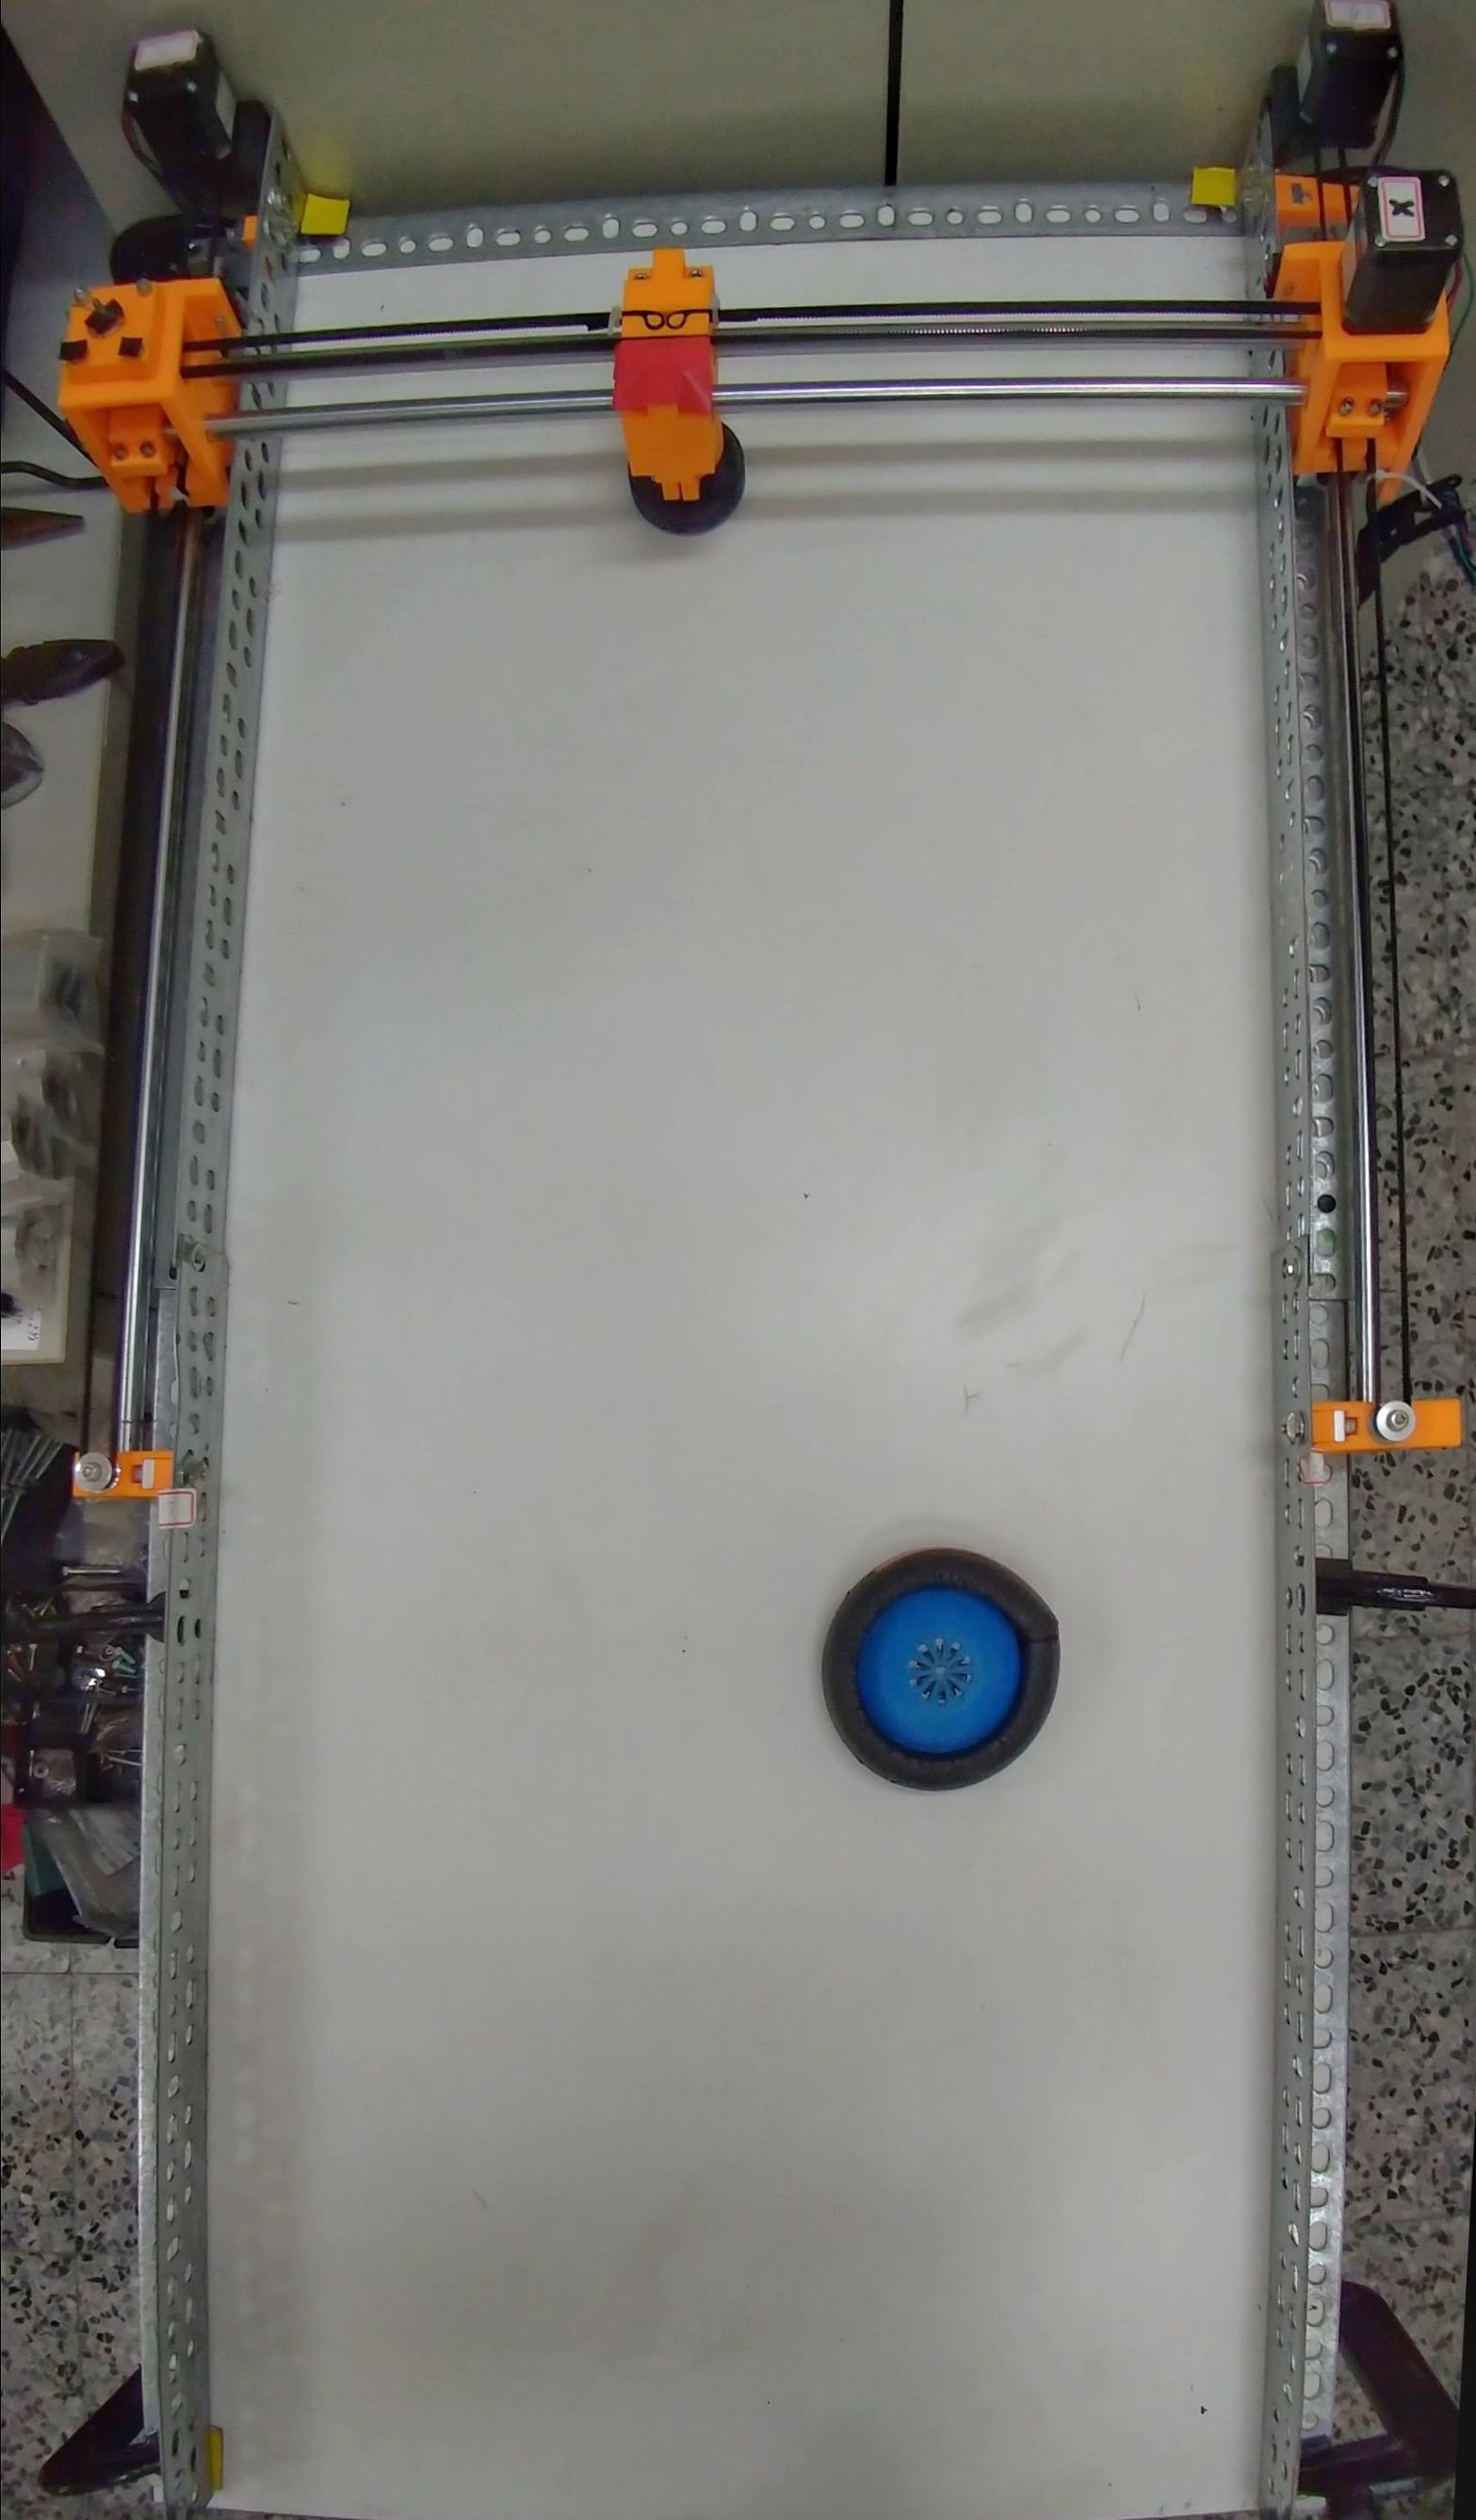
\includegraphics[width=3cm]{冰球機}
\caption{\Large 實體的冰球機}\label{fig.冰球機}
\end{center}
\end{figure}
\begin{figure}[hbt!]
\begin{center}
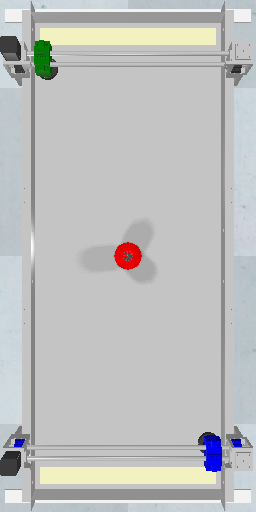
\includegraphics[width=3cm]{origin}
\caption{\Large 虛擬環境簡化後的冰球機}\label{fig.模擬冰球機}
\end{center}
\end{figure}
\begin{figure}[hbt!]
\begin{center}
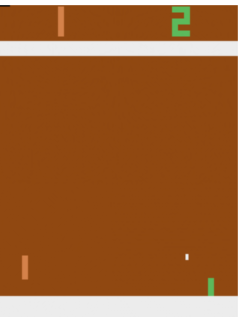
\includegraphics[width=3cm]{pong_gym}
\caption{\Large Gym的Pong game}\label{fig.pong_gym}
\end{center}
\end{figure}
